%%%%%%%%%%%%%%%%%%%%%%%%%%%%%%%%%%%%%%%%%%

\section{Results of the cut-based analysis}

\label{sec:results}

In this section we present the results of the 
cut-based analysis.
%
We present a detailed cut-flow for the various steps
of the analysis.
%
We
compare our results with other recent related studies, in particular
we study how the signal significance
is modified if only the $4b$ component of the
QCD multi-jet background is taken into account,
but the $2b2j$ and $4j$ components are neglected.
%


\subsection{Cut-flow and signal significance}

First of all, we compare the cross-sections at various
analysis levels for the three categories, for signal and background events,
by providing a detailed cut-flow.
%
We consider all backgrounds enumerated in Sect.~\ref{mcgeneration},
and also discuss how results are modified if only the $4b$
component is kept.
%
At each stage of the cut-flow, we also provide the
the signal significance, $S/\sqrt{B}$, and the signal
over background ratio, $S/B$, corresponding to the case of the
 HL-LHC with
an integrated luminosity of $\mathcal{L}_{\rm int}
=3000$ fb$^{-1}$.
%
We emphasize that it is important not only to achieve a good signal
significance, $S/\sqrt{B}$, but also a good signal over background ratio $S/B$:
if the latter is too small, a very accurate
measurement of the background with an infeasible small
systematic uncertainty would be required.


   

%%%%%%%%%%%%%%%%%%%%%%%%%%%%%%%%%%%%%%%%%%%%%%%%%%%%%%%%%%%%%%%%%%%%%%%%%%%%%%%%%%%%%%%%%
%%%%%%%%%%%%%%%%%%%%%%%%%%%%%%%%%%%%%%%%%%%%%%%%%%%%%%%%%%%%%%%%%%%%%%%%%%%%%%%%%%%%%%%%%
\begin{table}[t]
  \centering
  \begin{tabular}{|c|c|c|c|}
\hline
&  Boosted  &   Intermediate &  Resolved  \\
\hline
\hline
{\bf C0} &  \multicolumn{3}{c|}{Generator level} \\
\hline
{\bf C1a} & $N_{\rm jets}^{R10}\ge 2$ & $N_{\rm jets}^{R04}\ge 2$, $N_{\rm jets}^{R10}=1$  &
$N_{\rm jets}^{R04}\ge 4$ \\
\hline
{\bf  C1b} & \multicolumn{3}{c|}{+$p_T$ cuts} \\
{\bf C1c} & \multicolumn{3}{c|}{+rapidity cuts}\\
\hline
 {\bf C1d} & +$N_{\rm MDT}\ge 2$ & $N_{\rm jets}^{R10}=1$ with MDT  &
 Higgs reconstruction \\
 \hline
{\bf C1e} & \multicolumn{3}{c|}{ $m_H$ window cut} \\
\hline
{\bf C2} & \multicolumn{3}{c|}{$b$-tagging}    \\
\hline
  \end{tabular}
  \caption{\small Details of the cut-flow of the present analysis in the boosted, intermediate
    and resolved categories.
    %
      \label{tab:cutflowdetails}
  }
\end{table}
%%%%%%%%%%%%%%%%%%%%%%%%%%%%%%%%%%%%%%%%%%%%%%%%%%%%%%%%%%%%%%%%%%%%%%%%%%%%%%%%%%%%%%%%%
%%%%%%%%%%%%%%%%%%%%%%%%%%%%%%%%%%%%%%%%%%%%%%%%%%%%%%%%%%%%%%%%%%%%%%%%%%%%%%%%%%%%%%%%%


To begin with,
in Table~\ref{tab:cutflowdetails}
we summarize the details of the cut-flow of the present analysis,
separated into the exclusive boosted, intermediate
    and resolved categories.
    %
    From top to bottom, additional cuts are required in addition
    to the previous ones.
    %
    The various cuts
    are defined as follows
    \begin{itemize}
    \item {\bf C0}: these are the generator level cross-sections, with
      mild generation cuts in the case of the background processes, and no cuts
      for the signal events.
      %
    \item {\bf C1a}: at this level, we only check that we have at least
      two large-$R$ jets (in the boosted case),
      one large-$R$ jet and at least 2 small-$R$ jets (in the intermediate
      case) and at least four small-$R$ jets (in the resolved case).
      %
      No acceptance requirements are imposed here.
    \item {\bf C1b}: in addition, now the jets should
      satisfy the corresponding $p_T$ thresholds:
      $p_T \ge 200$ GeV for large-$R$ jets,
      $p_T \ge 50$ GeV for small-$R$ jets.
    \item {\bf C1c}: in addition, the above jets must satisfy the
      rapidity acceptance requirement.
    \item {\bf C1d}: at this level, the two leading large-$R$ jets must
      be mass-drop tagged in the boosted category.
      %
      In the intermediate category, the large-$R$ jet must also be mass-drop tagged.
      %
    \item {\bf C1e}: after the two Higgs candidate jets have been reconstructed,
      their invariant masses are required to lie a window around $m_H$,
      in particular between 100 and 150 GeV.
          \item {\bf C2}: This is the level of the analysis
            after $b$-tagging has been performed, using the strategy discussed
            in Sect.~\ref{sec:btagging}.
      \end{itemize}
    The signal and background events that satisfy all the analysis cut up to the
    C2 level
    are then used as input for the MVA training, as described next
    in Sect.~\ref{sec:mva}.

    %
    In Table~\ref{tab:cutflow_noPU_1} we provide
    the values of cross-sections, in femtobarns,
     for the signal
      and the various background
      components as a function of the
      cut-flow, for the resolved,
      boosted and intermediate
      categories.
      %
       In each case, we also provide the signal over
      background ratio, $S/B$, and the signal
      significance, $S/\sqrt{B}$, at the HL-LHC, considering either
      the total background or only the $4b$ component.
     %
      A first important observation from Table~\ref{tab:cutflow_noPU_1}
      is the role of the fake component of the QCD background.
      %
      We see that, even after $b$-tagging, the reducible $2b2j$ background
      is comparable or even larger, than the irreducible
      $4b$ component.
      %
      This is specially marked in the boosted category.
      %
      Therefore, at this level of the analysis, the signal significance
      can be artificially increased by up to a factor 2 if only the
      $4b$ background is considered.

      
    

%%%%%%%%%%%%%%%%%%%%%%%%%%%%%%%%%%%%%%%%%%%%%%%%%
\begin{table}[t]
  \centering
  \scriptsize
  \begin{tabular}{|l|cc|cccc|cccc|}
  \hline
\multicolumn{11}{|c|}{Resolved category, $\la n_{\rm PU}\ra=0$}\\
\hline
&  \multicolumn{6}{c|}{Cross-section [fb]} &  &  & &  \\
   &  $hh\to 4b$ &  total bkg  &   $4b$    &  $2b2j$   &   $4j$    &
$t\bar{t}$ &
$S/B_{\rm tot}$ & $S/B_{\rm 4b}$ & $S/\sqrt{B_{\rm tot}}$ & $S\sqrt{B_{\rm 4b}}$ \\
  \hline
  \hline
 C0    & $39$  &   $5.2\cdot 10^9$   & $1.8\cdot 10^6$ & $3.5\cdot 10^8$ & $4.9\cdot 10^9$ & $3.5\cdot 10^5$  & $7.5\cdot 10^{-9}$   &  $2.2\cdot 10^{-5}$  &   0.03   & 1.6        \\
 C1a   & $39$  &   $5.2\cdot 10^9$   & $1.8\cdot 10^6$ & $3.5\cdot 10^8$ & $4.9\cdot 10^9$ & $3.5\cdot 10^5$ &  $7.5\cdot 10^{-9}$   & $2.2\cdot 10^{-5}$   &     0.03   & 1.6       \\
 C1c   & $22$  &   $2.2\cdot 10^8$   & $6.9\cdot 10^4$ & $1.5\cdot 10^7$ & $2.0\cdot 10^8$ & $2.1\cdot 10^5$ &  $1.0\cdot 10^{-7}$  &  $3.2\cdot 10^{-4}$  &  0.08   & 4.6         \\
 C1d   & $22$  &   $2.2\cdot 10^8$   & $6.9\cdot 10^4$ & $1.5\cdot 10^7$ & $2.0\cdot 10^8$ & $2.1\cdot 10^5$ &  $1.0\cdot 10^{-7}$  & $3.2\cdot 10^{-4}$   &  0.08   & 4.6         \\
 C1e   & $63$  &   $4.4\cdot 10^7$   & $1.6\cdot 10^4$ & $3.2\cdot 10^6$ & $4.1\cdot 10^7$ & $8.8\cdot 10^4$ &   $1.4\cdot 10^{-7}$  &  $3.9\cdot 10^{-4}$   &   0.05   & 2.7         \\
 C2    & $1.2$  &   $4.9\cdot 10^3$   & $1.7\cdot 10^3$ & $2.9\cdot 10^3$ & $2.1\cdot 10^2$ & $47$ &            $ 2.5\cdot 10^{-4}$   & $7.1\cdot 10^{-4}$   &   0.97   & 1.6       \\
\hline
\end{tabular}

  $\,$ \\
  \vspace{0.5cm}
  \begin{tabular}{|l|cc|cccc|cccc|}
  \hline
\multicolumn{11}{|c|}{Intermediate category}\\
\hline
&  \multicolumn{6}{c|}{Cross-section [fb]} &  &  & &  \\
   &  $hh\to 4b$ &  total bkg  &   $4b$    &  $2b2j$   &   $4j$    &
$t\bar{t}$ &
$S/B_{\rm tot}$ & $S/B_{\rm 4b}$ & $S/\sqrt{B_{\rm tot}}$ & $S\sqrt{B_{\rm 4b}}$ \\
  \hline
  \hline
 C0      & 39  &   $5.2\cdot 10^9$   & $1.8\cdot 10^6$ & $3.5\cdot 10^8$ & $4.9\cdot 10^9$ & $3.5\cdot 10^5$ &  $7.5\cdot 10^{-9}$   & $2.2\cdot 10^{-5}$   &   $3.0\cdot 10^{-2}$   & 1.6  \\
 C1c     & 6.9  &   $8.4\cdot 10^7$   & $2.1\cdot 10^4$ & $5.3\cdot 10^6$ & $7.9\cdot 10^7$ & $3.3\cdot 10^4$ &  $8.2\cdot 10^{-8}$   & $3.3\cdot 10^{-4}$ &   $4.1\cdot 10^{-2}$   & 2.6 \\
 C1d     & 6.3  &   $5.8\cdot 10^7$   & $1.4\cdot 10^4$ & $3.6\cdot 10^6$ & $5.5\cdot 10^7$ & $3.0\cdot 10^4$ &  $1.1\cdot 10^{-7}$   & $4.6\cdot 10^{-4}$ &   $4.5\cdot 10^{-2}$   & 2.9\\
 C1e     & 1.3  &   $3.5\cdot 10^6$   & $8.7\cdot 10^2$ & $2.1\cdot 10^5$ & $4.3\cdot 10^7$ & $8.8\cdot 10^3$ &  $3.8\cdot 10^{-7}$   & $1.5\cdot 10^{-3}$  &   $3.9\cdot 10^{-2}$   & 2.5\\
 C2      & 0.22  &   $1.8\cdot 10^2$   & $5.6\cdot 10^1$ & $9.6\cdot 10^1$ & $2.2\cdot 10^1$ & 3.1 & $1.3\cdot 10^{-3}$   & $4.0\cdot 10^{-3}$  &   $9.2\cdot 10^{-1}$   & 1.6 \\
\hline
\end{tabular}

  $\,$ \\
  \vspace{0.5cm}
    \begin{tabular}{|l|cc|cccc|cccc|}
  \hline
\multicolumn{11}{|c|}{Boosted category, $\la n_{\rm PU}\ra=0$}\\
\hline
&  \multicolumn{6}{c|}{Cross-section [fb]} &  &  & &  \\
   &  $hh\to 4b$ &  total bkg  &   $4b$    &  $2b2j$   &   $4j$    &
$t\bar{t}$ &
$S/B_{\rm tot}$ & $S/B_{\rm 4b}$ & $S/\sqrt{B_{\rm tot}}$ & $S\sqrt{B_{\rm 4b}}$ \\
  \hline
  \hline
C0      & 39  &   $5.2\cdot 10^9$   & $1.8\cdot 10^6$ & $3.5\cdot 10^8$ & $4.9\cdot 10^9$ & $3.5\cdot 10^5$  &   $7.5\cdot 10^{-9}$   & $2.2\cdot 10^{-5}$  &  $ 3.0\cdot 10^{-2}$   & 1.6 \\
 C1a     & 39  &   $5.2\cdot 10^9$   & $1.8\cdot 10^6$ & $3.5\cdot 10^8$ & $4.9\cdot 10^9$ & $3.5\cdot 10^5$  &   $7.5\cdot 10^{-9}$   & $2.2\cdot 10^{-5}$ &  $ 3.0\cdot 10^{-2}$   & 1.6  \\
 C1c     & 9.4  &   $4.6\cdot 10^7$   & $1.1\cdot 10^4$ & $2.9\cdot 10^6$ & $4.3\cdot 10^7$ & $2.4\cdot 10^4$ &   $2.0\cdot 10^{-7}$   & $8.3\cdot 10^{-4}$ &  $ 7.6\cdot 10^{-2}$   & 4.8 \\
 C1d     & 6.7  &   $3.7\cdot 10^7$   & $7.5\cdot 10^3$ & $2.1\cdot 10^6$ & $3.5\cdot 10^7$ & $2.2\cdot 10^4$ &   $1.8\cdot 10^{-7}$   & $9.0\cdot 10^{-4}$ &  $ 6.0\cdot 10^{-2}$   & 4.2  \\
 C1e     & 2.5  &   $3.9\cdot 10^6$   & $8.0\cdot 10^2$ & $2.3\cdot 10^5$ & $3.7\cdot 10^6$ & $7.1\cdot 10^3$   &   $6.4\cdot 10^{-7}$   & $3.1\cdot 10^{-3}$ &  $ 6.9\cdot 10^{-2}$   & 4.9\\
 C2      & 0.4  &   $2.5\cdot 10^2$   & $5.3\cdot 10^1$ & $1.9\cdot 10^2$ & $1.3\cdot 10^1$ & 1.6  &   $1.4\cdot 10^{-3}$   & $6.7\cdot 10^{-3}$ &   1.2   & 2.7  \\
\hline
\end{tabular}
%%%%%%%%%%%%%%%%%%%%%%%%%%%%%%%%%%%%%%%%%%%%%%%%%%%%%%%%%%%%%%%

    \caption{\small The cross-sections, in femtobarns,
      for the signal and the various background
      processes at different steps of the
      cut-flow, for the resolved (upper table),
      intermediate (middle table) and boosted
      (lower table) categories, for the analysis
      without PU.
      %
      In each case, we also provide the signal over
      background ratio, $S/B$, and the signal
      significance, $S/\sqrt{B}$, considering either
      the total background or only the $4b$ component.
      %
      The different levels of the cut-flow are summarized
      in Table~\ref{tab:cutflowdetails}.
 \label{tab:cutflow_noPU_1}}
\end{table}
%%%%%%%%%%%%%%%%%%%%%%%%%%%%%%%%%%%%



%
In the boosted category, we see that after all the cuts, including $b$-tagging,
we end up with more than 1000 signal events at the HL-LHC, however swamped in a total
background of almost 1M QCD events.
%
This leads to a signal significance of around 1.0 at the end of the
cut-based analysis.
%
While it should have been possible to increase this significance
but using more aggressive cuts, we have refrained doing so
since we prefer this optimisation to be performed at the level of
the MVA.
%
We also note that $S/B$ is at the per-mille level, requiring a extremely accurate
measurement of the QCD background.


From the results of Table~\ref{tab:cutflow_noPU_1}
it is possible to compute the corresponding numbers
for the end of Run II at the LHC with
$\mathcal{L}_{\rm int}=300$ fb$^{-1}$: in the boosted category,
we have only
120 signal events, and the signal significance drops down to
$S/\sqrt{B}\sim 0.3$.
%
We will discuss in the next section what are the Run II prospects
once we include the effects of the MVA in the analysis, but
it is clear already at this level that one really needs the full
integrated luminosity of the HL-LHC to be able to observe
the Higgs pair production process, unless  of course production rates are
increased by new BSM dynamics

Both the intermediate and resolved categories benefit from higher signal yields,
specially in the resolved category, but this enhancement is compensated by the stronger
increase in the QCD multi-jet background.
%
In both cases the signal significance is similar to that of the boosted category,
with the additional drawback in the resolved case that the signal over background ratio
is one order to magnitude smaller.
%
Overall, we observe that 
that after the cut-based analysis,
the combination
of the boosted, intermediate and resolved categories yields
to total significance for the observation of the Higgs pair production
observation in the $b\bar{b}b\bar{b}$ final
state of around $S/\sqrt{B}=1.70$.

\subsection{The role of light jet mistags}

One of the main differences of the present study as compared
to previous works is the simulation of both irreducible
and reducible background components, which allows
to study the impact of the modeling of light and charm jet mistags. 
%
Now we compare our results with two recent studies that have also studied the
feasibility of SM Higgs pair production in the $4b$ final state,
those of the UCL group~\cite{Wardrope:2014kya} and of the
Durham group~\cite{deLima:2014dta}.
%
In the UCL group study~\cite{Wardrope:2014kya} is based
on requiring at least four $b$-tagged $R=0.4$ anti-$k_T$ jets
in the central acceptance with $p_T \ge 40$ GeV, which are
then used to form dijets (Higgs candidates) with
$p_T \ge 150$ GeV, $85 \le m_{\rm dijet} \le 140$ GeV
and $\Delta R \le 1.5$ between the two jets that form
each dijet system.
%
In addition to the basic selection cuts, a large number
of additional variables are combined using a
Boosted Decision Tree (BDT) discriminant.
%
This study considers the $b\bar{b}b\bar{b}$ and
$b\bar{b}c\bar{c}$ QCD multijets as well as
$t\bar{t}$, $Zh$, $t\bar{t}h$ and $hb\bar{b}$.
%
Their final significance is found to the $S/\sqrt{B}=2.1$ at the HL-LHC.

The Durham group study~\cite{deLima:2014dta} requires events
to have two $R=1.2$ C/A jets with $p_T\ge 200$ GeV, with
two $b$-tagged subjets inside each large-$R$ jet with
$p_T \ge$ 40 GeV.
%
To improve the signal over background separation, both the BDRS
method and the Shower Deconstruction (SD)~\cite{Soper:2011cr,Soper:2012pb}
technique are applied.
%
The background considered are QCD $4b$ as well as $Zb\bar{b}$, $hZ$ and
$hW$, but no $t\bar{t}$, $2b2j$ or $4j$.
%
At the HL-LHC, the best performance is obtained by requiring two
SD-tagged large-$R$ jets, which leads to $S/\sqrt{B}\sim 2.1$,
with BDRS similar but slightly inferior performance.
%
Therefore, both the Durham and the UCL groups conclude that a signal
significance $S/\sqrt{B}$ slightly above two can  be obtained
in this channel at the HL-LHC.

Since we find that the $2b2j$ and $4j$ backgrounds cannot
be neglected, and previous works did not considered them,
it is interesting to
study how our results are modified if we consider only the QCD $4b$
multi-jet background, but ignore the $2b2j$ and $4j$ backgrounds,
that is, we ignore the contribution from the fakes.
%
As we can seen before in Table~\ref{tab:cutflow_noPU_1},
these results indicate that given the similarity of the final states
in signal and background events in these cases, the signal significance is
relatively stable at various stages of the cut-flow.
%
As compared to the case in which all backgrounds are taken into account, we
now get a factor two smaller backgrounds: we conclude that in the boosted category
the effect of the fakes is non-negligible, with their contribution being
comparable to that of the irreducible $4b$ QCD multi-jet background.

Concerning the other categories, we see that that ignoring the fakes can lead to a substantial
distortion of the results.
%
In the intermediate category, the signal significance is now much better, with $S/\sqrt{B}$ increasing from
0.5 with all the backgrounds to $1.57$ if only $4b$ are accounted for, a factor 3 improvement.
%
Also the resolved category improves substantially, with signal significance increasing by a factor 2.
%
Therefore, we conclude that a careful modeling of the fakes is very important to truly quantify
the feasibility of Higgs pair production in the $4b$ channel, though for the most
important category, the boosted category, the results are relatively stable.
%
Moreover, we find that the effect of the multijet fake background is of
the same size of the higher-order QCD corrections to $4b$ production~\cite{Binoth:2009rv}.



In summary, we find that the results of our cut-based analysis are roughly
consistent with the results of previous related studies.
%
Indeed, combining the signal significance in the three categories, we end
up with a final $S/\sqrt{B}\simeq 2.3$.
%
As we show next, once the MVA is used, we achieve a substantial
improvement
over previous works, even after taking into account our rather more
complete modelling of the QCD multijet background.



In Table~\ref{tab:cutflow_noPU_1}   we show the results for the cross-sections for the different
backgrounds that we consider at the end of the cut-based analysis, for each
of the three categories.
%
Recall that all the backgrounds have been normalized to known higher-order results,
as summarized in Table~\ref{tab:samples}.
%
As we can see from this comparison, as opposed that what naively one would expect,
the QCD $2b2j$ background turns out not to be negligible as compared to the $4b$
multijets in any of the categories.


In the boosted case, the sum of the $2b2j$ and $4j$ components is almost as large as the
irreducible $4b$ background, thus increasing the total background rates by a factor 2 as compared
to the case where only $4b$ is accounted for.
%
This effect is more dramatic in the intermediate and resolved categories: in the former,
$2b2j$ completely dominates the background (thus the increase in $S/\sqrt{B}$
obtained when only the $4b$ component is kept), and in the latter
it is comparable to $4b$.
%
Therefore, we conclude that an accurate estimate of the fake $b$-tag contribution is
an essential component of this analyses, and that complete QCD multijet samples
should be included.
%
On the other hand, we find that the hadronic $t\bar{t}$ component of the background
is smaller than the QCD multijet one.

In Fig.~\ref{fig:histoBack} we show the decomposition of the background for one important kinematical
distribution, the $p_T$ of the leading reconstructed Higgs candidate, various background
components, for both the boosted and the resolved categories.
%
In the same figure we also show the results of the corresponding comparison
at the level of the $p_T^{hh}$ of the
reconstructed di-Higgs system.
%
The histograms correspond to the distributions at the end of the cut-based
analysis.
%
The results are consistent with those summarized
before in the boosted case we see how $4b$ is the most important
component of the background, with $2b2j$ being of the same order of magnitude, while
for the resolved category we see that $2b2j$ dominates instead.
%
So the effect of the fakes is certainly important, but fortunately it is not a limiting factor
in the resolved category, the one that leads to higher signal significance.

%%%%%%%%%%%%%%%%%%%%%%%%%%%%
\begin{figure}[t]
\begin{center}
 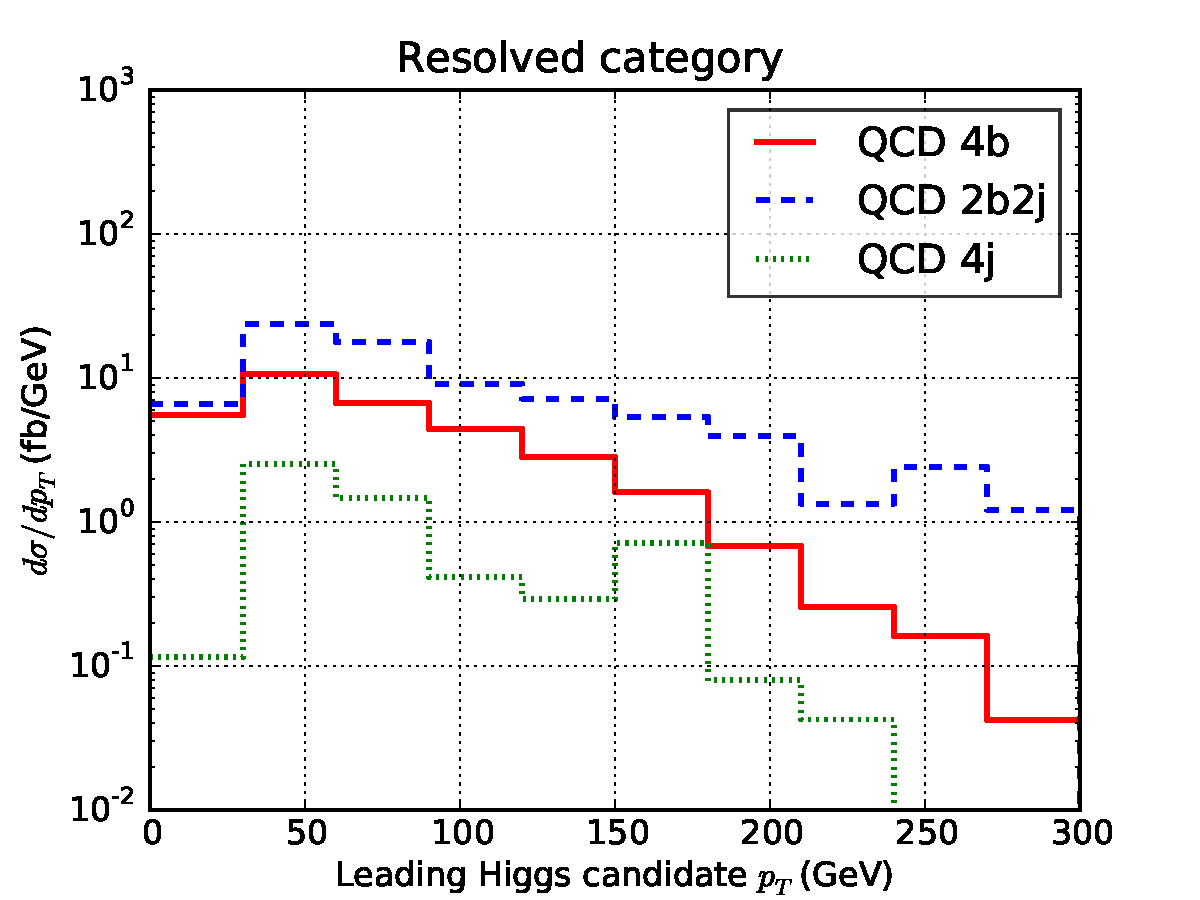
\includegraphics[width=0.49\textwidth]{plots/pt_H0_C2_res_back.pdf}
 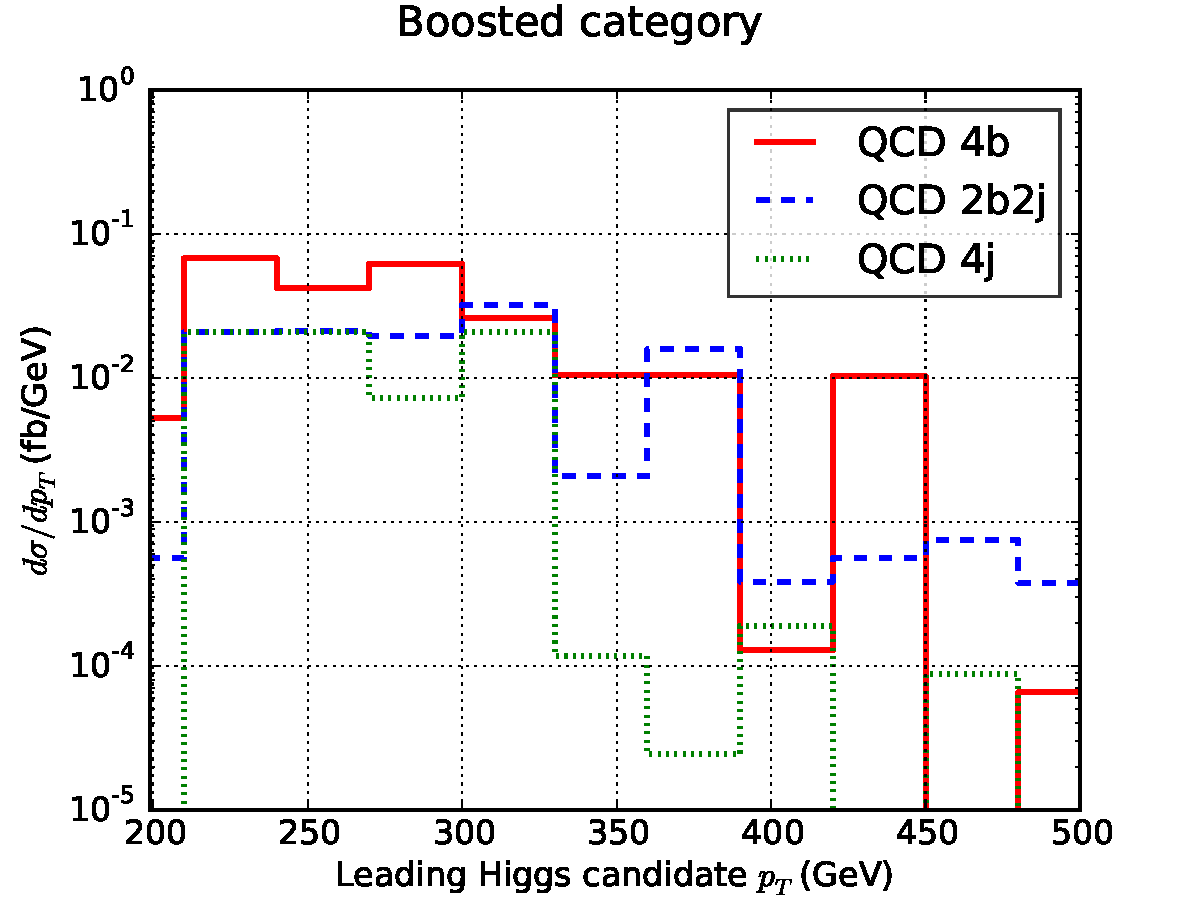
\includegraphics[width=0.49\textwidth]{plots/pt_H0_C2_boost_back.pdf}
   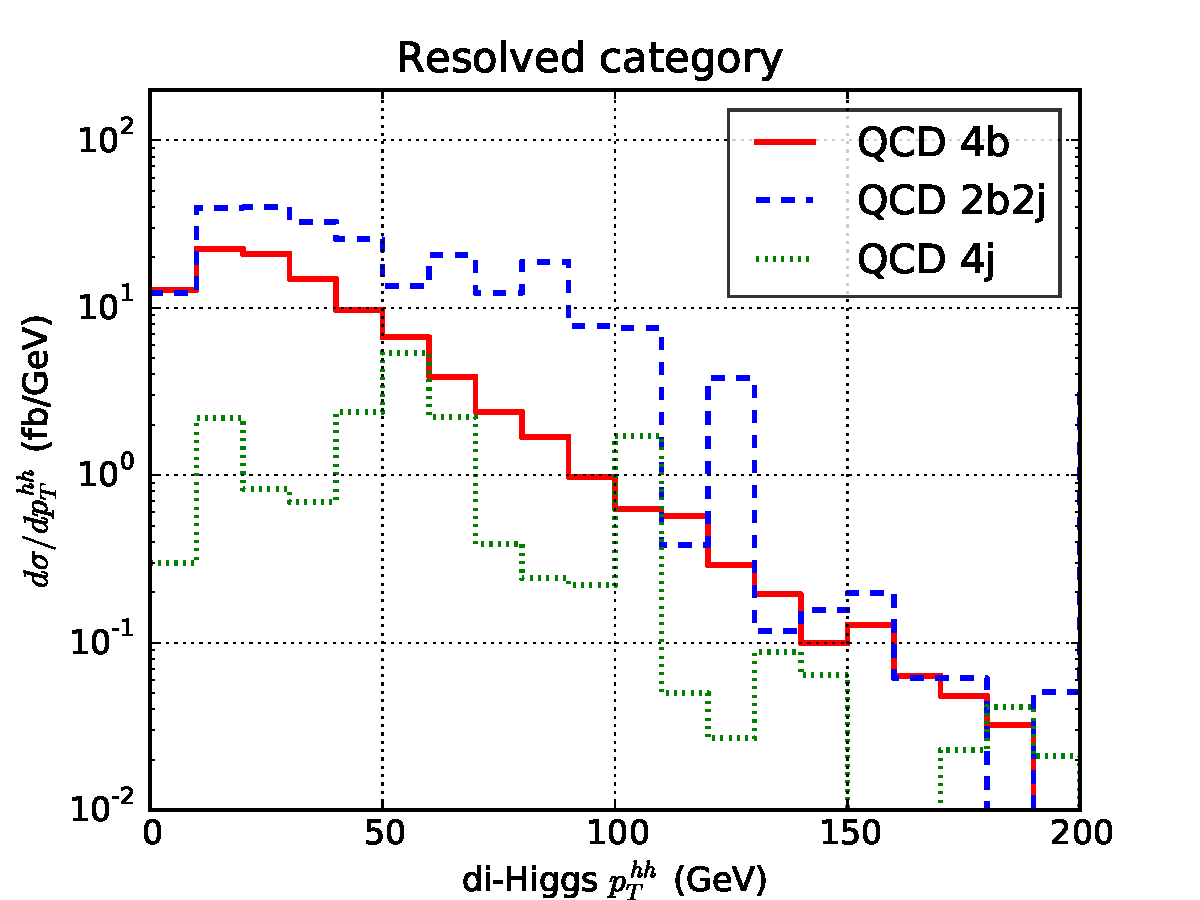
\includegraphics[width=0.49\textwidth]{plots/pt_HH_C2_res_back.pdf}
  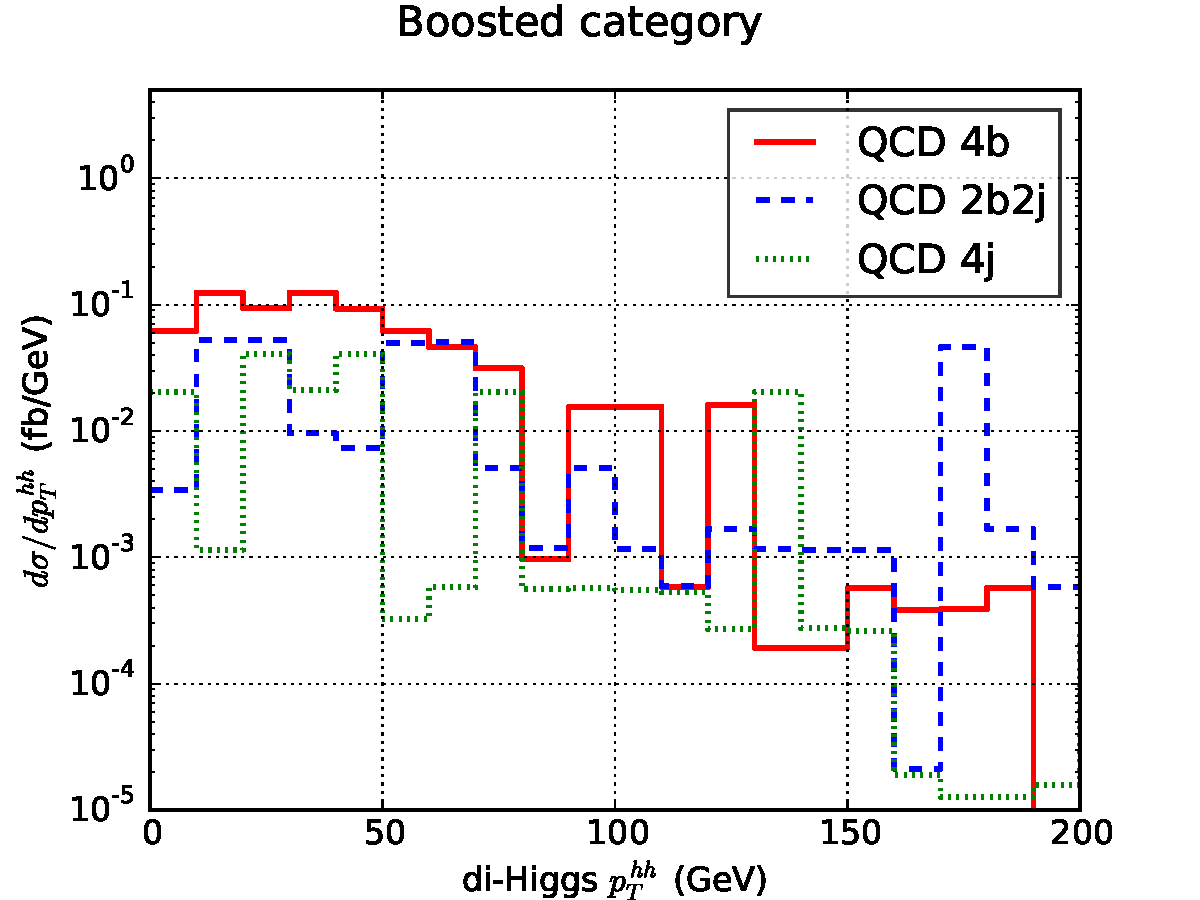
\includegraphics[width=0.49\textwidth]{plots/pt_HH_C2_boost_back.pdf}
  \caption{\small
    Upper plots: the decomposition of the QCD multijet background in its various
    components, $4b$, $2b2j$ and $4j$, for the $p_T$ of the leading
    Higgs candidate in the boosted (left plot) and resolved (right plot) categories.
    %
    Lower plots: the same comparison this time for the $p_T^{hh}$ of the
    reconstructed di-Higgs system.
}
\label{fig:histoBack}
\end{center}
\end{figure}
%%%%%%%%%%%%%%%%%%%%%%%

  One might ask why the $2b2j$ process
  is not subdominant as compared to $4b$: while its generator-level cross-section is
  much larger, $\sigma_{2b2j} \simeq 240\cdot \sigma_{4b}$, one expects a suppression
  of the order of $f_l^2 =10^{-4}$ since only with two light jets mistagged as $b$-jets the event
  would be identified as a Higgs candidate.
  %
  We have checked that this expectation is true only at parton level: once parton shower effects
  are accounted for, both the radiation of $b\bar{b}$ pairs from the shower and combinatorics increase
  the number of $b$ quarks in the final state, enhancing substantially the $2b2j$ rates as compared
  to the naive parton level expectation.
  %





